\setcounter{chapter}{12-1}

\chapter{Clustering}

    \subsection{Why do clustering?}
    
        In chapter 4, we discussed \textbf{classification}: sorting data points into different groups, or \textbf{classes}. 
        
        \miniex We might sort animals by \textbf{genetics}, or different sub-diseases that need different \textbf{treatments}. 
        
        \textbf{Simplifying} our data into \textbf{categories} can allow us to do better work, more easily.
        
        This has lots of benefits: 
        
        \begin{itemize}
            \item It could be used to make \textbf{decisions}. Sometimes, knowing the class of an object is enough to make a decision, by itself.
        
            \item We could use this to understand the structure and \textbf{distribution} of our data.
            
            \item We could sort different types of data to be processed \textbf{separately}.
        \end{itemize}
        
        The problem is, this relied on us \textbf{knowing} what classes we plan to sort into. 
        
        This may seem obvious, but what if we're looking at something \textbf{new}? A disease we don't fully \textbf{understand}, or animals we've never seen before? How do we classify them?
        
        In the past, we've done this ourselves, giving us lots of useful classifications. But, computers allow us to do this in new situations:
        
        \begin{itemize}
            \item \textbf{High-dimensional} datasets, with too much \textbf{complex} information for a human to make sense of.
                \begin{itemize}
                    \item \miniex Looking for patterns in hundreds of genetic factors at the same time.
                \end{itemize}
            
            \item Discovering new classes \textbf{faster} than ever using computers.
                \begin{itemize}
                    \item And thus saving human labor.
                \end{itemize}
            
            \item Finding \textbf{patterns} in creative ways humans would never think to, especially for really \textbf{abstract} problems.\\
        \end{itemize}
    
        \begin{concept}
            \vocab{Clustering} is like \purp{classification}, where we want to assign things to \gren{classes}: we call them \vocab{clusters}.
            
            But, we use it when we \purp{don't know} what groupings we want, so we have to \gren{find} them.
        \end{concept}
        
        We have some challenges ahead of us, though. How do we decide what things are "similar" or "different"? How do we create new classes, and know that they're meaningful?
        
        

\pagebreak
%%%%%%%%%%%%%%%%%%%%%%%%%%%%%%%%%%%%%%%%%%%%%%%%%%%%%%%%%%%%%%%%%%%%%%%%%%%%%

\section{Clustering Formalisms}

    \subsection{Unsupervised Learning}
        
        The first thing we should note: 
        
        This problem is similar to classification, a \textbf{supervised} problem.
        
        It was \textbf{supervised} because we knew the \textbf{correct} labels for our data in our advance. We just wanted to \textbf{teach} it to our computer.
        
        The problem here: we \textbf{don't} know the correct labels! In fact, we're making them up as we go. Because we aren't being "supervised" by a correct answer, we call this \textbf{unsupervised learning}.\\
        
        \begin{concept}
            \vocab{Clustering} is a type of \purp{unsupervised learning}: meaning, we don't have a \gren{correct} answer in advance.
            
            The labels we create are not based on a \purp{known} truth.
            
            The \gren{label} for data point $\ex{x}{i}$ is written as $\ex{y}{i}$.
        \end{concept}
        
    \subsection{What is clustering?}
    
        So, if we don't know \textbf{what} our classes are, how do we figure out \textbf{which} classes to create?
        
        Intuitively, we think of classes as a \textbf{collection} of things that are \textbf{similar} to each other. Before, we've considered things "\textbf{close}" if they have a \textbf{low distance} in input space.
            \note{Remember that input space is where we represent each data point using input variables.}
            
        \miniex We can tell two animals are \textbf{both} cats because they both have fur and sharp claws, among other things: they're \textbf{similar}.
            
        Meanwhile, two points in different classes are more \textbf{different}: they're further apart in input space. 
        
        \miniex We can tell a dolphin is \textbf{distinct} from a cat because one lives in water and one doesn't: their clusters are more \textbf{different}.
        
        We call each of these groupings \textbf{clusters}.\\
        
        \begin{definition}
            Informally, a \vocab{cluster} is a collection of \gren{data points} that are all 
            \begin{itemize}
                \item \purp{Near} each other
                
                \item \purp{Far} from the other clusters.
            \end{itemize}
            
            We use clusters as our way to \gren{discover} new classifications.
        \end{definition}
        
        \miniex Below, we can visually mark out what looks like 5 distinct \textbf{clusters} in input space $(x_1,x_2) \in \RR^2$:
        
        \begin{figure}[H]
            \centering
            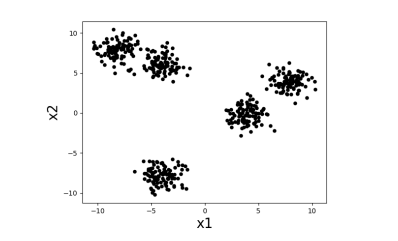
\includegraphics[width=70mm,scale=0.4]{images/clustering_images/clustering_example.png}
        \end{figure}
        
        This is an informal way to understand clusters, though. If we want to be more precise, we need to ask ourselves questions like:
        
        \begin{itemize}
            \item What does it mean for points to be "close" or "far"? How are we measuring distance?
            
            \item How many clusters do we want?
            
            \item How do we evaluate our clustering?
        \end{itemize}
        
\pagebreak
%%%%%%%%%%%%%%%%%%%%%%%%%%%%%%%%%%%%%%%%%%%%%%%%%%%%%%%%%%%%%%%%%%%%%%%%%%%%%

\section{The k-means formulations}

    In this section, we'll introduce a common way to do clustering called the \textbf{$k$-means approach}.

    \subsection{Defining a cluster: The mean}
        
        We need to define what makes a "cluster" in order to move \textbf{forward}.
        
        We want the points within a cluster to be as \textbf{close together} as possible. So, you might measure the \textbf{distance} from one point to all the others.
        
        So, it would make sense to \textbf{average} them out. And we need to average every pair of points. That's a lot of work: can we \textbf{simplify} it?
        
        Well, if we're trying to \textbf{average} the result of many data points, it would make sense to use the \textbf{mean}!
        
        That's how we'll \textbf{define} our cluster: as the \textbf{mean}, the point that is the \textbf{average} of all the other points in the cluster.\\
        
        \begin{definition}
            We want to represent our \purp{cluster} using its \vocab{mean}: the \gren{average} of all of the data points in that \purp{cluster}.
             
            Our goal is for the \vocab{cluster mean} to have the \vocab{minimum average distance} possible to all of our data points: it's as \gren{close} to our points as we can get.
        \end{definition}
        
        \miniex We describe the "male lifespan" using \textbf{life expectancy}: the \textbf{average} time a male human lives for. Same for women as well.
         
    \subsection{$k$-means}
    
        Now, we've created \textbf{one} cluster. To extend this to \textbf{many} clusters, we just need each cluster to have its \textbf{own} mean.
        
        There are $k$ of these clusters: this is why we call this the \textbf{k-means formulation}.
        
        How do we decide which point goes in which \textbf{cluster}? Well, we want our points to be close. So, we'll assign it to the \textbf{closest} one.\\
        
        \begin{concept}
            A \gren{point} is assigned to the \purp{closest} \vocab{cluster mean}.
            
            For a point $\ex{x}{i}$, the \gren{output} is which \purp{cluster} ("new class") it has been assigned to: $\ex{y}{i}$.
        \end{concept}
        
        Once we've successfully clustered using our \textbf{algorithm} below, we will find that both of these goals are met:
        
        \begin{itemize}
            \item Our points are \textbf{assigned} to the \textbf{closest} cluster mean.
            
                \begin{itemize}
                    \item This separates \vocab{different} clusters of points from each other.
                \end{itemize}
            
            \item The cluster mean is the \textbf{average} of all of our points: the \textbf{minimum distance} to them.
            
                \begin{itemize}
                    \item This makes sure our cluster is made up of points that are \vocab{similar} to each other.
                    
                    \item If our point is close to the \textbf{mean}, it's probably close to the \textbf{other} points in the cluster.
                \end{itemize}
        \end{itemize}
        
    \subsection{$k$-means loss}
    
        Now, we know what we want out of our \textbf{clusters}. But, the problem is, we don't know \textbf{which} points will give us our nice clusters. 
        
        So, first, we will have to \textbf{assign} our initial "cluster means": often, we \textbf{randomly} select some points from our dataset.\\
        
        \begin{concept}
            We \vocab{initialize} our clustering by \purp{randomly} selecting one point to \gren{represent} each cluster, which we call the \vocab{cluster mean}.
            
            At first, each point is assigned to the \purp{closest} cluster mean.
        \end{concept}
        
        But as you'll notice, these points are \textbf{not} the cluster means we're looking for! They're just a random \textbf{initialization}. So, we have to \textbf{optimize}.\\
        
        \begin{clarification}
            Notice that, when we \gren{first} select our "cluster means", we don't get them by \purp{averaging} any points: we choose them \purp{randomly}.
            
            That means, at first, is our cluster mean \vocab{isn't a true mean}!
            
            Our $k$-means algorithm is designed to \gren{fix} this problem.
        \end{clarification}

        
        In order to \textbf{improve} our clustering, it helps to have a way to measure the \textbf{quality} of a clustering: we need a \textbf{loss function}.
    
    \subsection{One-cluster loss}
    
        Let's start with just one cluster: what do we want to \textbf{minimize}? 
        
        Well, we want the points within a cluster to be as \textbf{close together} as possible. So, we want to minimize the \textbf{distance} to the mean, $\mu$.
        
        To make our function smooth, we'll use \textbf{squared distance} instead.\\
        
        \begin{concept}
            In \vocab{k-means loss}, we want to minimize the \purp{square distance} from each point $\ex{x}{i}$ to the \gren{cluster mean} $\mu$.
        \end{concept}
        
        \begin{equation}
            D_i = \norm{ \rxi - \blu{\mu} }^2
        \end{equation}
        
        We'll add this up for each of the $n$ data points in our cluster.
        
        \begin{equation}
            \loss = \sum_{i=1}^n \norm{ \rxi - \blu{\mu} }^2
        \end{equation}
        
    \subsection{Building up to $k$ clusters}
    
        So, what do we do for each of our $k$ clusters? Well, we can just \textbf{add} up the \textbf{loss} for them.
        
        We'll use $j \in \{1, 2, 3, ... k\}$ to represent our $\nth{j}$ cluster. Each cluster has a mean $\blu{\ex{\mu}{j}}$.
        
        %%%%%%%%%%%%%%%%%%%%%%%%%%%%%%%%%%%%%%%%% Command for readability
        \newcommand{\bmuj}[0]{ \blu{\ex{\mu}{j}} } %Blue mu^j
        %%%%%%%%%%%%%%%%%%%%%%%%%%%%%%%%%%%%%%%%%
        
        \begin{equation}
            \loss_j = \sum_{i=1}^n \norm{ \rxi - \bmuj }^2
        \end{equation}
        
        Problem is, we're including \textbf{every} point $\exi$ in \textbf{every} cluster! We want a way to filter by \textbf{cluster}.
        
        Remember that we \textbf{label} clusters the same way we labeled \textbf{classes} before:\\
        
        \begin{notation}
            For a \vocab{data point} $\exi$, its \purp{cluster} is given by
            
            \begin{equation*}
                \eyi \in \{1, 2, ... k \}
            \end{equation*}
            
            Where $j$ represents the $\nth{j}$ cluster.
        \end{notation}
        
        Cluster mean $\bmuj$ is the $\nth{j}$ cluster mean: it only counts for points in $c_j$. So, we \textbf{only} want to add up the loss when 
        
        \begin{equation}
            \eyi = j
        \end{equation}
        
        We'll do this using the following helpful \textbf{function}:\\
        
        \begin{notation}
            The \vocab{indicator function} $\mathbb{1}$ tells you whether a statement $p$ is true:
            
            \begin{equation*}
                \mathbb{1}(p) = 
                \begin{cases}
                    1 & \text{if $p$} \\
                    0 & \text{otherwise }
                \end{cases}
            \end{equation*}
        \end{notation}
        
        Combined with our \textbf{condition} of matching clusters, this can be useful:
        
        \begin{equation}
            \mathbb{1}(\eyi = j)
        \end{equation}
        
        If we \textbf{multiply} this by our loss, it'll \textbf{only} appear if the clusters \textbf{match}! We can \textbf{eliminate} data points in a different cluster.
        
    \subsection{$k$-mean loss: final form}
    
        So, we can \textbf{filter} by the data points in our cluster:
        
        \begin{equation}
            \loss_j =
            \sum_{i=1}^n 
                \overbrace{
                    \mathbb{1}(\eyi = j)
                }^{ \text{Check cluster}}
                \overbrace{
                    \norm{ \rxi - \bmuj }^2 
                }^{\text{Sq. dist from mean} }
        \end{equation}
        
        And finally, we add up over many clusters:
        
        \begin{equation}
            \loss = \sum_{j=1}^k \loss_j
        \end{equation}
        
        Using our equation, we get:
        
        \begin{equation*}
                \loss =
                \overbrace{
                    \sum_{j=1}^k
                }^{\text{clusters }}
                \overbrace{
                \sum_{i=1}^n 
                }^{\text{data points}}
                    \overbrace{
                        \mathbb{1}(\eyi = j)
                    }^{ \text{Check cluster}}
                    \overbrace{
                        \norm{ \rxi - \bmuj }^2 
                    }^{\text{Dist from mean} }
            \end{equation*}
            
            Let's clean that up:\\
        
        \begin{kequation}
            The \vocab{$k$-means loss} is given as:
            
            \begin{equation*}
                \loss =
                \pur{
                    \sum_{j=1}^k \sum_{i=1}^n
                }
                \red{
                    \mathbb{1}(\eyi = j)
                }
                \blu{
                    \norm{ \exi - \bmuj }^2 
                }
            \end{equation*}
            
            Where:
            
            \begin{itemize}
                \item $\mu_j$ is the \vocab{cluster mean}: the \purp{average} of the points in the $\nth{j}$ cluster.
                
                \item $\mathbb{1}(\eyi = j)$ is the \vocab{indicator function}: meaning that we only \gren{include} terms where the data point and mean are in the \purp{same cluster}.
            \end{itemize}
        \end{kequation}
        
        
    \subsection{Making further use of the indicator function (Optional)}
        
        We can actually use our \textbf{indicator function} to represent some of our \textbf{other} variables:
        
        For example: the \textbf{cluster mean} is the average of data points, but \textbf{only} those belonging to that cluster. 
        
        So, we can use $1(\cdot)$ to \textbf{filter} those other data points out:
        
        \begin{equation}
            \ex{\mu}{j} = \frac{1}{N_j} 
            \sum_{j=1}^k 
                \overbrace{
                    \mathbb{1}(\eyi = j)
                }^{ \text{check cluster} }
                \overbrace{
                    \exi
                }^{ \text{data points} }
        \end{equation}
        
        And how large is $N_j$? We can just \textbf{add} 1 for every data point in cluster, 0 otherwise:
        
        \begin{equation}
            N_j = 
            \sum_{j=1}^k 
                \mathbb{1}(\eyi = j)
        \end{equation}
        
        One more loose end: we've been focusing on \textbf{square distance} as loss function. We want to minimize this, but we're doing this over multiple data points.
        
        So, really we want to minimize the \textbf{average} of that. This is a very common (and very useful!) property of a distribution called the \textbf{variance}.\\
        
        \begin{definition}
            The \vocab{variance} of a dataset is the \vocab{average square distance} from the \purp{mean}:
            
            \begin{equation*}
                \operatorname{Var}[X] = \frac{1}{N} \sum_{i=1}^{N} (\ex{x}{i} - \mu)^2
            \end{equation*}

            It tells us how \gren{spread out} our data is.
        \end{definition}
        
        That means, our loss function is meant minimize the total \textbf{variance}.
            \note{Almost, the factor of $1/N$ is missing: since this won't change as we improve our clustering, we'll leave it alone.}
            
    \subsection{Initializing the $k$-means algorithm}
    
        Now that we have our \textbf{clusters}, \textbf{means}, and a \textbf{loss} function for evaluating them, we can begin looking for a better \textbf{clustering}.
        
        We'll start out with a \textbf{dataset} we want to cluster: we'll use the one from the \textbf{beginning} of the chapter:
        
        \begin{figure}[H]
            \centering
            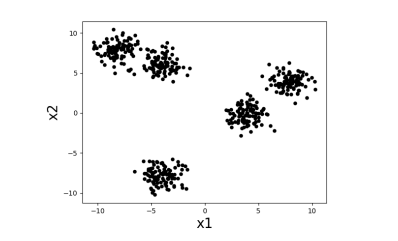
\includegraphics[width=70mm,scale=0.4]{images/clustering_images/clustering_example.png}
            \caption*{We could cluster this visually, but we want our machine to be able to do it for us.}
        \end{figure}
        
        First, we need to decide on our \textbf{number} of clusters. When you can't \textbf{visualize} it, this can be \textbf{difficult} - how many is too many or too few? 
        
        But, for now, we'll \textbf{ignore} that problem, and say $k=5$. 
        
        Let's \textbf{randomly} assign our initial cluster means, and assign each point to the \textbf{closest} cluster:
        
        \begin{figure}[H]
            \centering
            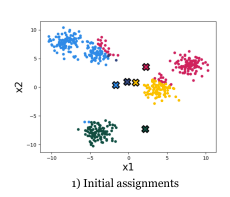
\includegraphics[width=70mm,scale=0.4]{images/clustering_images/initialization_cluster.png}
            \caption*{This is our starting point for the algorithm.}
        \end{figure}
    
    \subsection{First step: moving our cluster means}
    
        As we mentioned before, these points aren't \textbf{actually} the average of their cluster: you can tell that by looking at it.
        
        We want to \textbf{minimize} the variation in our cluster: that's why we're using the mean.
        
        So, let's fix this: we'll take the \textbf{average} of all the points in each \textbf{cluster}, and \textbf{move} the cluster mean to that position.
        
        \begin{figure}[H]
            \centering
            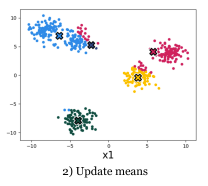
\includegraphics[width=70mm,scale=0.4]{images/clustering_images/update_means_clustering.png}
        \end{figure}
        
        And now, our cluster means are closer to all our data points!\\
        
        \begin{concept}
            One way \vocab{minimize} the \vocab{distance} between the \purp{cluster mean} and its \gren{data points} is:
            
            \begin{itemize}
                \item Take the \gren{average} of all the points in the cluster, and \purp{reassign} the cluster mean to that average.
            \end{itemize} 
        \end{concept}
        
    \subsection{Second step: Reassign data points}
    
        We've \textbf{improved} our model by moving the cluster mean.
        
        The problem is, we originally \textbf{assigned} every point to the \textbf{closest} cluster mean. 
        
        If the cluster means \textbf{move}, then some points might be closer to a \textbf{different} cluster now!
        
        If so, we can \textbf{improve} our clustering further by reassigning points to the cluster they're \textbf{closest} to!
        
        \begin{figure}[H]
            \centering
            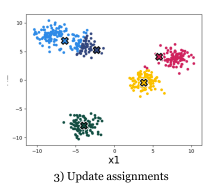
\includegraphics[width=70mm,scale=0.4]{images/clustering_images/update_assignments_clustering.png}
        \end{figure}\\
        
        \begin{concept}
            Another way \vocab{minimize} the \vocab{distance} between the \purp{cluster mean} and its \gren{data points} is:
            
            \begin{itemize}
                \item After the \purp{means} have been \gren{moved}, \vocab{reassign} the \vocab{data points} to whichever mean is \purp{closest}.
            \end{itemize} 
        \end{concept}
        
    \subsection{The cycle continues}
    
        But wait - now that we've changed the points in each cluster, our cluster mean might not be the \textbf{true} average!
        
        So, we can, again, improve our loss by taking the average of each cluster, and moving the cluster mean.
        
        This creates a cycle that continues until we \textbf{converge} on our final answer.\\
        
        \begin{concept}
            Together, of our steps for \gren{improving} our clusters create a \vocab{cycle} of \purp{optimization}:
            
            \begin{itemize}
                \item \purp{Moving} our cluster mean \gren{changes} which point should go in each cluster.
                
                \item \purp{Reassigning} points to different clusters \gren{changes} our cluster mean.
            \end{itemize}
        \end{concept}
        
    \subsection{The $k$-means algorithm}
    
        These two steps make up the \textbf{bulk} of our algorithm:\\
        
        \begin{definition}
            The \vocab{$k$-means algorithm} uses the following steps:
            
            \begin{itemize}
                \item First, we \purp{randomly} choose our \gren{initial} cluster means.
            \end{itemize} 
            
            Then, we \purp{cycle} through the following two steps:
            
            \begin{itemize}
                \item \purp{Reassign} \gren{points} to the cluster mean they're closest to.
                
                \item \purp{Move} each \gren{cluster mean} to the average of all the points in that cluster.
            \end{itemize}
            
            Until our clusters means \purp{stop} changing.
        \end{definition}
        
        When we run our algorithm on the above dataset, we get:
        
        \begin{figure}[H]
            \centering
            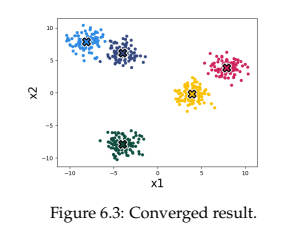
\includegraphics[width=70mm,scale=0.4]{images/clustering_images/converged_result_clustering.png}
        \end{figure}
        
        Note that, our cycle \textbf{works} because changing \textbf{either} cluster mean or point assignments allows you to further \textbf{improve} the \textbf{other} step.
        
        So, if we're \textbf{not} changing one of them, the other one won't \textbf{change} either: the cycle is \textbf{broken}, and we can \textbf{stop}. 
            \note{This is our termination condition!}
        
        Another nice fact: it can be shown that this algorithm does \textbf{converge} to a local minimum!\\
        
        \begin{concept}
            The \vocab{$k$-means algorithm} is guaranteed to \purp{converge} to a \gren{local minimum}.
        \end{concept}
        
    \subsection{Pseudocode}
    
        \begin{codebox}
          \Procname{$\proc{k-means}(k, \tau, \{x^{(i)}\}_{i=1}^n)$}
          \li $\mu, y \gets $ randinit  \qquad\#Random initialization
          \li \For $t \gets 1$ \To $\tau$   \qquad\#Begin cycling
          \li
          \li   \Do
                 $y_{\texttt{old}} = y$ \qquad\#Keep track of last step
                 
          \li
          \li        \For $i \gets 1$ \To $n$
          \li       \Do
                     $y^{(i)} = \arg\min_j \left\Vert x^{(i)} - \mu^{(j)} \right\Vert_2^2$
                     \qquad\#Reassign data point to closest mean
                    \End
                    
          \li
          \li    \For $j \gets 1$ \To $k$
          \li       \Do 
                     $\mu^{(j)} = \frac{1}{N_j} \sum_{i=1}^n \mathbb{1}(y^{(i)} = j) x^{(i)}$
                     \qquad\#Move cluster mean to average of cluster
                    \End
                    
        \li
          \li      \If $\mathbb{1}(y = y_{\texttt{old}})$
          \li          \Then
        		  break \qquad\#If nothing has changed, then the cycle is done. Terminate
              \End
              \End
          \li
          \li \Return $\mu, y$
        \end{codebox}
        
    \subsection{Using gradient descent: minimizing distance to $\mu$}
    
        We can also use \textbf{gradient descent} to solve this problem!
        
        We want to \textbf{minimize} our loss $\loss$, and we do this by \textbf{adjusting} our cluster means $\ex{\mu}{j}$ until they're in the \textbf{best} position.\\
        
        \begin{concept}
            We can solve the \vocab{$k$-means problem} using \vocab{gradient descent}!
        \end{concept}
        
        So, we want to \textbf{optimize} $\loss$ using $\mu$:
        
        \begin{equation}
            \loss(\mu) =
            \sum_{i=1}^n 
                    \mathbb{1}(\eyi = j)
                    \norm{ \rxi - \bmuj }^2 
        \end{equation}
        
        Rather than dealing with the indicator function $1(\cdot)$, we could instead just consider whichever $\mu$ is closest: \textbf{minimum} distance.
        
        \begin{equation}
            \overbrace{
                \min_{j} 
            }^{Minimizing}
            \overbrace{
                \norm{ \rxi - \bmuj }^2 
            }^{distance}
        \end{equation}
        
        This \textbf{automatically} assigns every point to the closest \textbf{cluster} before we get our loss! So, all we need to worry about is $\mu_j$.
        
        \begin{notation}
            Instead of using an \purp{indicator function}, we can represent \gren{cluster assignment} another way: using the \vocab{function} $\min_{j}$.
            
            It can give \vocab{minimum distance} from $\ex{x}{i}$ to one of the cluster means: it picks the \purp{closest} mean. 
            
            This \gren{automatically} assigns the point to the \purp{closest} cluster, making our job easier.
        \end{notation}
        
        \begin{equation}
            \loss(\mu) =
            \sum_{i=1}^n 
            \overbrace{
                    \min_{j} 
            }^{\text{Nearest cluster}}
                    \norm{ \rxi - \bmuj }^2 
        \end{equation}
        
        Now, we can do gradient descent using $\pderiv{L(\mu)}{\mu}$. 
            \note{We move our means until they're minima!}
        
        $L(\mu)$ is \textbf{mostly} smooth, except when the cluster assignment of a \textbf{point} changes. So, it's usually smooth \textbf{enough} to do gradient descent.
    
    \subsection{Getting labels}
        
        Once we've finished gradient descent, and we've \textbf{minimized} our loss, we can get our \textbf{labels}.
        
        $\min$ gives the \textbf{output} value that we get by minimizing. In this case, average \textbf{squared distance} from the cluster mean.
        
        Meanwhile, $\argmin$ gives us the \textbf{input} value that gives us the minimum output. In this case, the \textbf{cluster} that gives the minimum distance. 
        
        So, $\argmin$ gives us the cluster closest to each point: that's our \textbf{label}!
        
        We can use this notation to get our \textbf{labels}.\\
        
        \begin{notation}
            After \purp{optimizing} $\mu$, our \vocab{labels} are given by:
            
            \begin{equation}
                \eyi = \arg\min_j \norm{ x^{(i)} - \mu^{(j)} }^2
            \end{equation}
        \end{notation}
        
        Using gradient descent can give us a \textbf{local} minimum, but our surface is not fully \textbf{convex}: so, we don't necessarily get a \textbf{global} minimum.
            \note{Even though individual terms of squared distance may be convex, adding $\min$ terms may not be convex.}

\pagebreak
%%%%%%%%%%%%%%%%%%%%%%%%%%%%%%%%%%%%%%%%%%%%%%%%%%%%%%%%%%%%%%%%%%%%%%%%%%%%%

\section{How to evaluate clustering algorithms}

    The biggest problem with clustering algorithms is that they're \textbf{unsupervised}: this makes it much harder to know if we've gotten a \textbf{good} result.
    
    This is partly because our \textbf{loss} function doesn't necessarily tell us if clustering is \textbf{useful}, or represents the data \textbf{accurately}.
    
    It just tells us if our points are \textbf{close} to their cluster \textbf{mean}. That doesn't always mean the clustering is \textbf{good}.
    
    \miniex Imagine \textbf{every} single point in the dataset gets its \textbf{own} cluster mean. The \textbf{distance} to the cluster mean would be 0 (low loss), but this isn't very \textbf{useful}!
        \note{This isn't useful because nothing has changed: we've gone from having $n$ separate data points, to having... $n$ separate clusters.}\\
    
    \begin{clarification}
        The \vocab{$k$-means loss function} does \purp{not} tell us if we have a good and \gren{useful} clustering or not.
        
        It only tells us if the points in our clusters are \purp{close} to their \gren{cluster mean}.
        
        This can help us make \purp{better} clusters, but that does not mean they are \gren{good} or what we \gren{want}.
    \end{clarification}
    
    Without having "true" labels, we have to find other ways to \textbf{verify} our approach.
    
    We'll do two things to \textbf{approach} this problem:
    
    \begin{itemize}
        \item We'll look at some of the ways our \textbf{algorithm} can go wrong (or right).
        
        \item Then, we'll find \textbf{better} ways to evaluate our clusterings than just looking at the \textbf{loss}.
    \end{itemize}
    
    But, always remember that a "good" clustering is partly \textbf{subjective}, and depends on what you \textbf{want} to accomplish.

    \subsection{Initialization}
    
        The first problem we have is related to something we mentioned at the end of the last section: $k$-means is not \textbf{convex}. 
        
        That means we can find \textbf{local} minima that are not the \textbf{global} minimum: our \textbf{initialization} (our \textbf{starting} clusters) can affect whether we end up in a useful minimum.
            \note{The reason why is, mathematically, the same as when we first introduced the idea of a local minimum.}
            
        \begin{figure}[H]
            \centering
            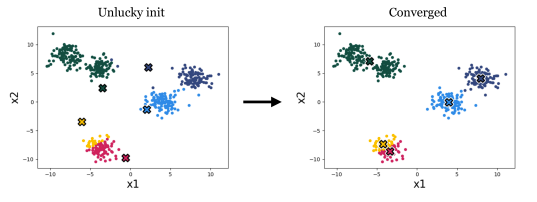
\includegraphics[width=100mm,scale=0.4]{images/clustering_images/unlucky_init.png}
            \caption*{In this example, notice that we ended up with convergence on some very \textbf{bad} clusters: the bottom cluster is split in \textbf{half}!}
        \end{figure}
        
        The easiest way to resolve this is to run $k$-means multiple times with different initializations.
            \note{Other techniques exist, but this is the simplest one.}\\
        
        \begin{concept}
            Getting an \vocab{unlucky initialization} can result in \purp{clusters} that aren't \gren{useful}.
            
            We try to \gren{solve} this by running our algorithm \purp{multiple times}.
        \end{concept}
        
        
    \subsection{Choice of $k$}
    
        One important question we decided to \textbf{ignore} earlier was: \textbf{how many} clusters should we pick in advance?
        
        Especially for \textbf{complex} data, we \textbf{don't know} how many natural clusters there will be. 
        
        But our number of clusters matter: because it's a parameter determines \textbf{how} our learning algorithm runs (rather than being chosen \textit{by} the algorithm), it's a \textbf{hyperparameter}:\\
        
        \begin{concept}
            Our \vocab{number of clusters} $k$ is a \vocab{hyperparameter}.
        \end{concept}
        
        And, choosing too high \textit{or} too low can both be \textbf{problematic}:
        
        \begin{itemize}
            \item If we set $k$ too \textbf{high}, then we have more clusters than actually \textbf{exist}.
                \begin{itemize}
                    \item This can cause us to \textbf{split} real clusters in half, or find \textbf{patterns} that don't exist.
                    
                    \item In a way, this resembles a kind of \textbf{overfitting}: we try to \textbf{closely} match the data, but end up fitting \textbf{too closely} and not \textbf{generalizing} well: \textbf{estimation error}.
                    
                    \item \miniex The \textbf{extreme} case looks like the example we mentioned \textbf{before}: when labeling animals, we could make... a different \textbf{species} for every single instance of \textbf{any} animal we find. 
                        \note{That doesn't sound very helpful.}
                \end{itemize}
            \item If we set $k$ too \textbf{low}, we don't have \textbf{enough} clusters to represent our data.
                \begin{itemize}
                    \item This means some clusters will be \textbf{lumped together} as a single thing: we \textbf{lose} some information.
                    
                    \item In this case, it's \textbf{impossible} to cluster everything in the way that would make the most \textbf{sense}: we have \textbf{structural error}.
                    
                    \item \miniex Let's say we wanted to \textbf{sort} fish, birds, and mammals into \textbf{two} categories: we might just \textbf{divide} them into "flies" and "doesn't fly".
                        \note{That's some information, but often not enough!}\\
                \end{itemize}
        \end{itemize}
        
        \begin{concept}
            When choosing $k$ (our \vocab{number of clusters}), we can cause \purp{problems} by picking an inappropriate \gren{value}:
            
            \begin{itemize}
                \item \vocab{Too many} clusters (large $k$) can cause \gren{overfitting} and \purp{estimation error}: we find patterns we don't want.
                
                \item \vocab{Not enough} clusters (small $k$) causes \purp{structural error}: it prevents us from correctly \gren{separating} data.
            \end{itemize}
        \end{concept}
        
    \subsection{Subjectivity of $k$}
    
        Not only is it hard to choose a "good" value of $k$, what a good value of $k$ is can really depend on your opinion, and what you know about reality.
        
        For example, consider the following example:
        
        \begin{figure}[H]
            \centering
            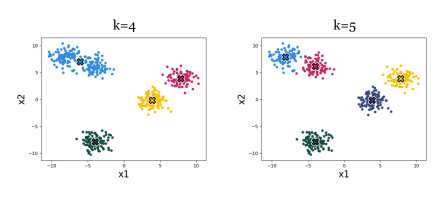
\includegraphics[width=100mm,scale=0.4]{images/clustering_images/subjective_k_value.png}
            \caption*{Which of these two clusterings is more accurate?}
        \end{figure}
        
        Should the top left be \textbf{one} cluster, or \textbf{two}? It's hard to say!
        
        Even if you're \textbf{sure}, you might \textbf{disagree} with others, or find that the best one depends on your \textbf{needs}.
        
        So not only can $k$ values be too high or too low, they can also be \textbf{debatably} better or worse!
        
        \begin{concept}
            The \vocab{best} choice of \vocab{clustering} is not entirely objective: it can depend on your \gren{opinion}, or how you plan to \purp{use} the clustering.
        \end{concept}
        
        What do we mean by, what we're "\textbf{using}" the clustering for? We'll get into that later, but in short: we might use \textbf{clusters} to make sense of \textbf{information}, or to make better \textbf{decisions}. 
        
        Different clusterings might be good when you want a different kind of understanding.
        
        \miniex The understanding you get from high-level comparisons (plants vs animals vs bacteria) is different from low-level comparison (cats vs dogs).
    
    \subsection{Hierarchical Clustering}
    
        That last example reveals something: not all types of groups are the same! Some are much broader than others, for example.
        
        If two types of groups are different, then why do we only have to have one type in our clustering? We don't have to restrict ourselves to a single $k$.
        
        Instead, we could treat some groups as inside of other groups: we call this a \textit{hierarchy}, because some groups are "higher" on the scale.\\
        
        \begin{definition}
            \vocab{Hierarchical Clustering} is when we cluster at multiple different \purp{levels}. 
            
            Some groups are \vocab{high-level}, or \purp{coarse}: they are groupings that contains \gren{more elements}: items in the same group can be more \purp{different}.
            
            Some groups are \vocab{low-level}, or \purp{fine}: they are groupings that contain \gren{fewer elements}: items in the same group have to be very \purp{similar}.
        \end{definition}
        
        \miniex Categorizing living things is done using hierarchical clustering: some groupings \textbf{contain} other groupings.
        
        \begin{figure}[H]
            \centering
            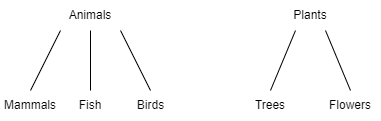
\includegraphics[width=70mm,scale=0.4]{images/clustering_images/hierarchical_life.png}
            \caption*{The top row of clusters are more \textbf{coarse}, while the bottom row is more \textbf{fine}.}
        \end{figure}
        
        We can \textbf{split} our groupings into \textbf{smaller} and smaller ones, to be as \textbf{fine-grained} as we need. Useful!

    \subsection{$k$-means in feature space}
        
        One \textbf{important} consideration: when working with \textbf{feature} representations, we found that sometimes, feature transformations made it \textbf{easier} to \textbf{classify} data.
            \note{Often, it wasn't even possible without those transformations!}
            
        Clustering is very \textbf{similar}, so, could we do the same here? It turns out, we \textbf{can}!
        
        Rather than directly clustering in \textbf{input} space $x$, we can \textbf{process} our data using features, and then cluster in \textbf{feature} space $\phi(x)$.\\
        
        \begin{concept}
            \vocab{Feature transformations} can be used to make it easier to \purp{accurately} cluster our data in a \gren{meaningful} way.
        \end{concept}
        
        There are some \textbf{other} reasons to do feature transformations, though: imagine that our data is \textbf{stretched} out along axis $x_1$, but not $x_2$.
        
        %Figure?
        
        $x_1$ distances would be \textbf{larger} in general: it would contribute more to our distance metric! We could correct for this by \textbf{standardizing} our data: \textbf{scaling down} the more stretched axis.
        
        This would be a \textbf{feature} transformation, and would make it \textbf{easier} to do our \textbf{clustering}.
    
    \subsection{Solutions: Validation}
    
        Now, we start trying to answer the \textbf{question}: how do we \textbf{check} whether we have a \textbf{good} clustering?
        
        Well, first, we can check for a \textbf{poor fit} (or overfitting) using new, \textbf{held-out} testing data: do we get \textbf{low loss} on that testing data?
        
        If we \textbf{don't}, then our clusters definitely aren't \textbf{representative} of the overall \textbf{dataset}: they don't \textbf{generalize} to new data.\\
        
        \begin{concept}
            If our clusters give \gren{large} \vocab{testing loss}, then they aren't \purp{generalizing} well, and are probably \gren{not representative} of the overall distribution.
            
            So, we already know our clusters \vocab{don't fit the distribution}.
        \end{concept}
        
            
    \subsection{Solutions: Consistency}
    
        But, just like for classification/regression \textbf{validation}, we don't only run our algorithm \textbf{one time}: we'll run it \textbf{many} times, with different training and testing sets.
        
        We can't \textbf{just} use the loss, though: having \textbf{more} clusters could make our error lower, without making a better clustering, for example.
        
        Another thought: we're trying to find some patterns \textbf{inherent} in the data. The idea is: if the pattern we're finding is \textbf{real}, we should find a similar pattern \textbf{each time}!
        
        So, we look to see if our clusters are \textbf{consistent} when we generate them using different training data: 
            \note{Different training data from the same distribution, of course.}
        if they \textbf{aren't}, then it's possible we're not finding the "\textbf{real}" patterns in the data.\\
        
        \begin{concept}
            If our \vocab{clusters} accurately \purp{reflect} the underlying classes of data, then we should expect some \vocab{consistency} of which clusters we \gren{generate} by running $k$-means many times.
            
            If our clusters aren't \purp{consistent}, then we might doubt if any of them especially reflect the \purp{distribution}, rather than \gren{noise}.
        \end{concept}

        If our clusters are \textbf{consistent}, then we're probably seeing something about the \textbf{real} dataset.
            \note{If it was based on random noise, then the odds of getting matching results would be really low!}
    
    \subsection{Solutions: Ground Truth}
    
        But, even if we're getting something \textbf{consistent}, that doesn't mean we're seeing the patterns that \textbf{matter}. 
        
        One way to \textbf{check} this is, if we have some idea of what the "\textbf{true}" clustering looks like for just a few data points, we can compare those results to ours.
        
        We call this "real" clustering the "ground truth".\\
        
        \begin{definition}
            In machine learning, the \vocab{ground truth} is what we know about the "real world".
            
            In general, we want our models to be able to \purp{reproduce} this reality: it is the data that we tend to \gren{trust} the most, if it is gathered correctly.
        \end{definition}
        
        That way, we can use a very \textbf{small} amount of \textbf{supervision} to get an idea of whether our clustering is on the \textbf{right track}.
    
    \subsection{Applications: Visualization and Interpretability}
    
        We've discussed some ways to \textbf{abstractly} test whether our clustering might be \textbf{accurate} the data.
        
        But, when it comes down to it, often, the \textbf{quality} of a clustering is based on how \textbf{useful} it is. So, what sorts of \textbf{uses} does clustering \textbf{have}? 
        
        Well, we're organizing our data into \textbf{groups}: this \textbf{simplifies} how we look at our data. And it allows us to \textbf{view} at our data, and \textbf{understand} what's going on.
        
        In short: clustering allows humans to more easily make sense of data.\\
        
        \begin{concept}
            One of the the main \gren{goals} of \vocab{clustering} is to make it easier for humans to \purp{understand} the data.
            
            This happens in two ways:
            
            \begin{itemize}
                \item We can \vocab{visualize} the data: we can \gren{see} it, and more easily use our \purp{intuition} to make sense of it.
                
                \item We can \vocab{interpret} our data: by seeing what sorts of \gren{groupings} we create, we learn about the \purp{structure} of the data.
            \end{itemize}
        \end{concept}
        
        So, machine learning experts judge partly based on how well a clustering \textbf{helps} them \textbf{achieve} these two goals.
        
        \textbf{Evaluating} clusterings is \textbf{subjective} for exactly this reason: what is \textbf{good} "visually", or is the \textbf{best} "interpretation" of data, is often up to \textbf{debate}.
        
        So, \textbf{human} judgement is important for this type of \textbf{problem}.
    
    \subsection{Applications: Downstream Tasks}
    
        Finally, there's one more way to think about clustering that is more \textbf{practical}, and closer to \textbf{objective}.
        
        We use clustering to \textbf{sort} different data points that need \textbf{different} processing: this can make our model more \textbf{effective}, since different parts of the dataset may work \textbf{better} with different \textbf{treatment}.
        
        \miniex We could train a different regression model on each cluster: this can create a more accurate model.
        
        We call this next problem a \textbf{downstream application}.\\
        
        \begin{definition}
            A \vocab{downstream application} is a \gren{problem} that relies on a \purp{different} process to make its work better or easier.
            
            In this case, \gren{clustering} has \purp{downstream applications} that can \gren{take advantage} of the \purp{structure} it reveals.
        \end{definition}
        
        If our clustering is \textbf{good}, we would expect it to \textbf{improve} the performance of downstream tasks.\\
        
        \begin{concept}
            We can indirectly \vocab{evaluate} a \purp{clustering algorithm} based on how \gren{successful} the \vocab{downstream application} is.
            
            If it \gren{improves} the performance of a downstream application, we could say it works \purp{well}.
        \end{concept}
        
    \subsection{A benefit of clustering}
    
        One advantage for downstream applications is, there might be patterns that are more obvious if you only look at related segment of the data. For example:
        
        \begin{figure}[h]
            \centering
            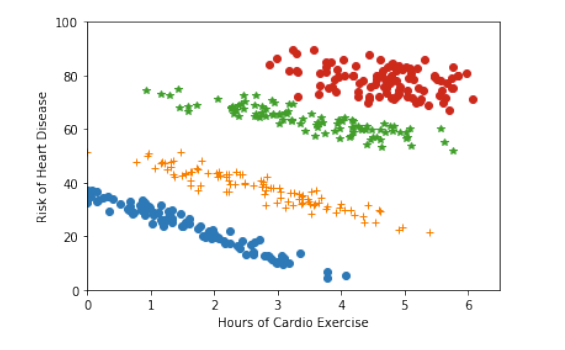
\includegraphics[width=0.65\textwidth]{images/clustering_images/simpsons_problem.png}
        \end{figure}
        
        If we take the data as a whole (\textbf{no} clustering), we would draw a \textbf{positive} regression: it seems that exercise and heart disease increase \textbf{together}. That doesn't make sense!
        
        But, if we divide it into \textbf{clusters}, based on age, we see a \textbf{negative} relationship: each individual group experiences \textbf{benefits} from exercise.
        
        This particular issue is called \textbf{Simpson's Paradox}.\\
        
        \begin{definition}
            \vocab{Simpson's Paradox} is when a \purp{trend} that appears in groups of data either \gren{vanishes} or \gren{reverses} when we look at all the data \purp{together}.
            
            It shows that sometimes, \purp{patterns} that we see may reflect how we're \gren{looking} at the data.
        \end{definition}
        
        Rest assured, you don't need to know this paradox by \textbf{name}! But it's important to \textbf{understand} possible problems like it: it'll make you more \textbf{responsible} in the future!
        
    \subsection{Weaknesses of $k$-means}
    
        %%%%%%%%%%%%%%%%%%%%%%%%%%
        %Future edit: explain *why* these shapes cause issues: low variance expects a blob
        %Also show sine waves, parallel lines as examples
        %%%%%%%%%%%%%%%%%%%%%%%%%%
    
        There are some \textbf{weaknesses} to $k$-means clustering. Certain patterns that we can \textbf{see} aren't easily \textbf{clustered}.
        
        We can see this with a few \textbf{examples}:
        
        \begin{figure}[h]
            \centering
            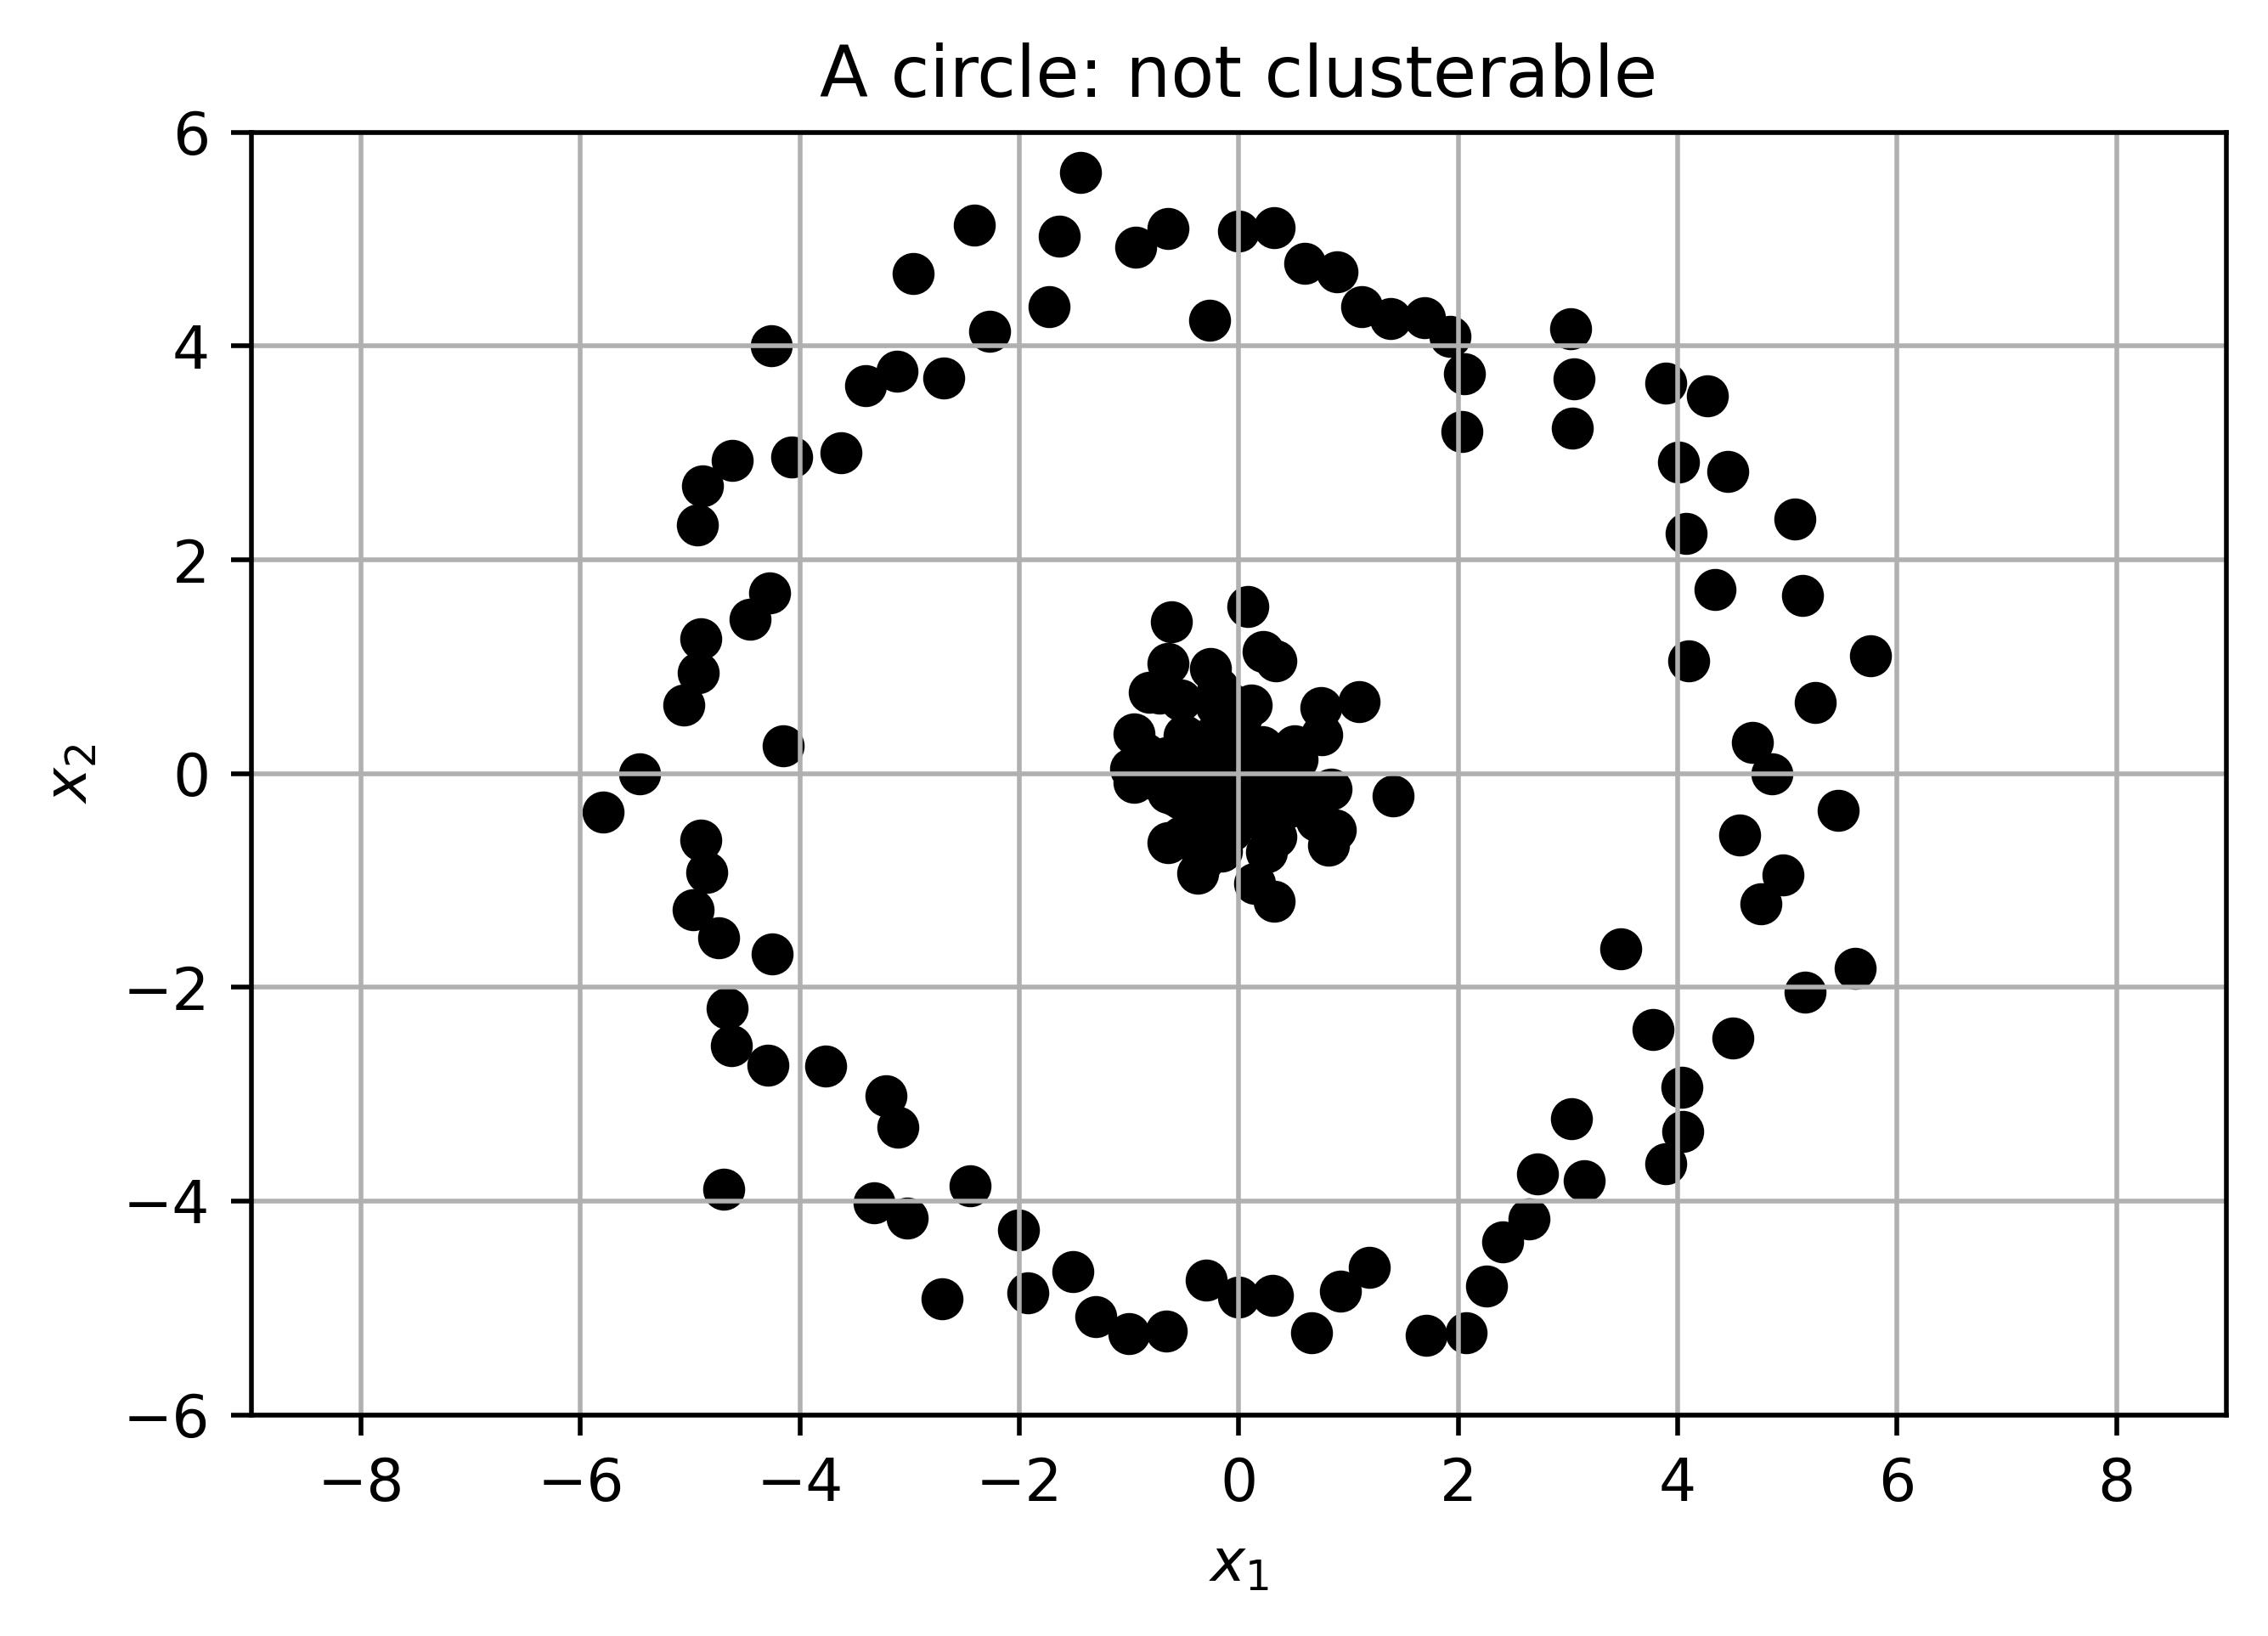
\includegraphics[width=0.65\textwidth]{images/clustering_images/center_unclusterable.png}
            \caption*{This data can't be simply clustered.}
        \end{figure}
        
        This example can't be effectively \textbf{clustered}: most people would agree that the "outer ring" should be \textbf{one} cluster, while the "inner circle" should be \textbf{another}.
        
        But, assuming we (correctly) place one cluster mean in the \textbf{center}, there's \textbf{nowhere} we can put our other cluster mean to be \textbf{closest} to all of the \textbf{outer} points, but \textbf{not} the inner points.
        
        We might be able to \textbf{resolve} this using a \textbf{feature} transformation. But, the problem remains.
            \note{For example, we could have a feature represent the radius! But then, we would still struggle with a ring not centered on the origin.}
            
        Another example works for clusters that aren't very centralized:
        
        \begin{figure}[h]
            \centering
            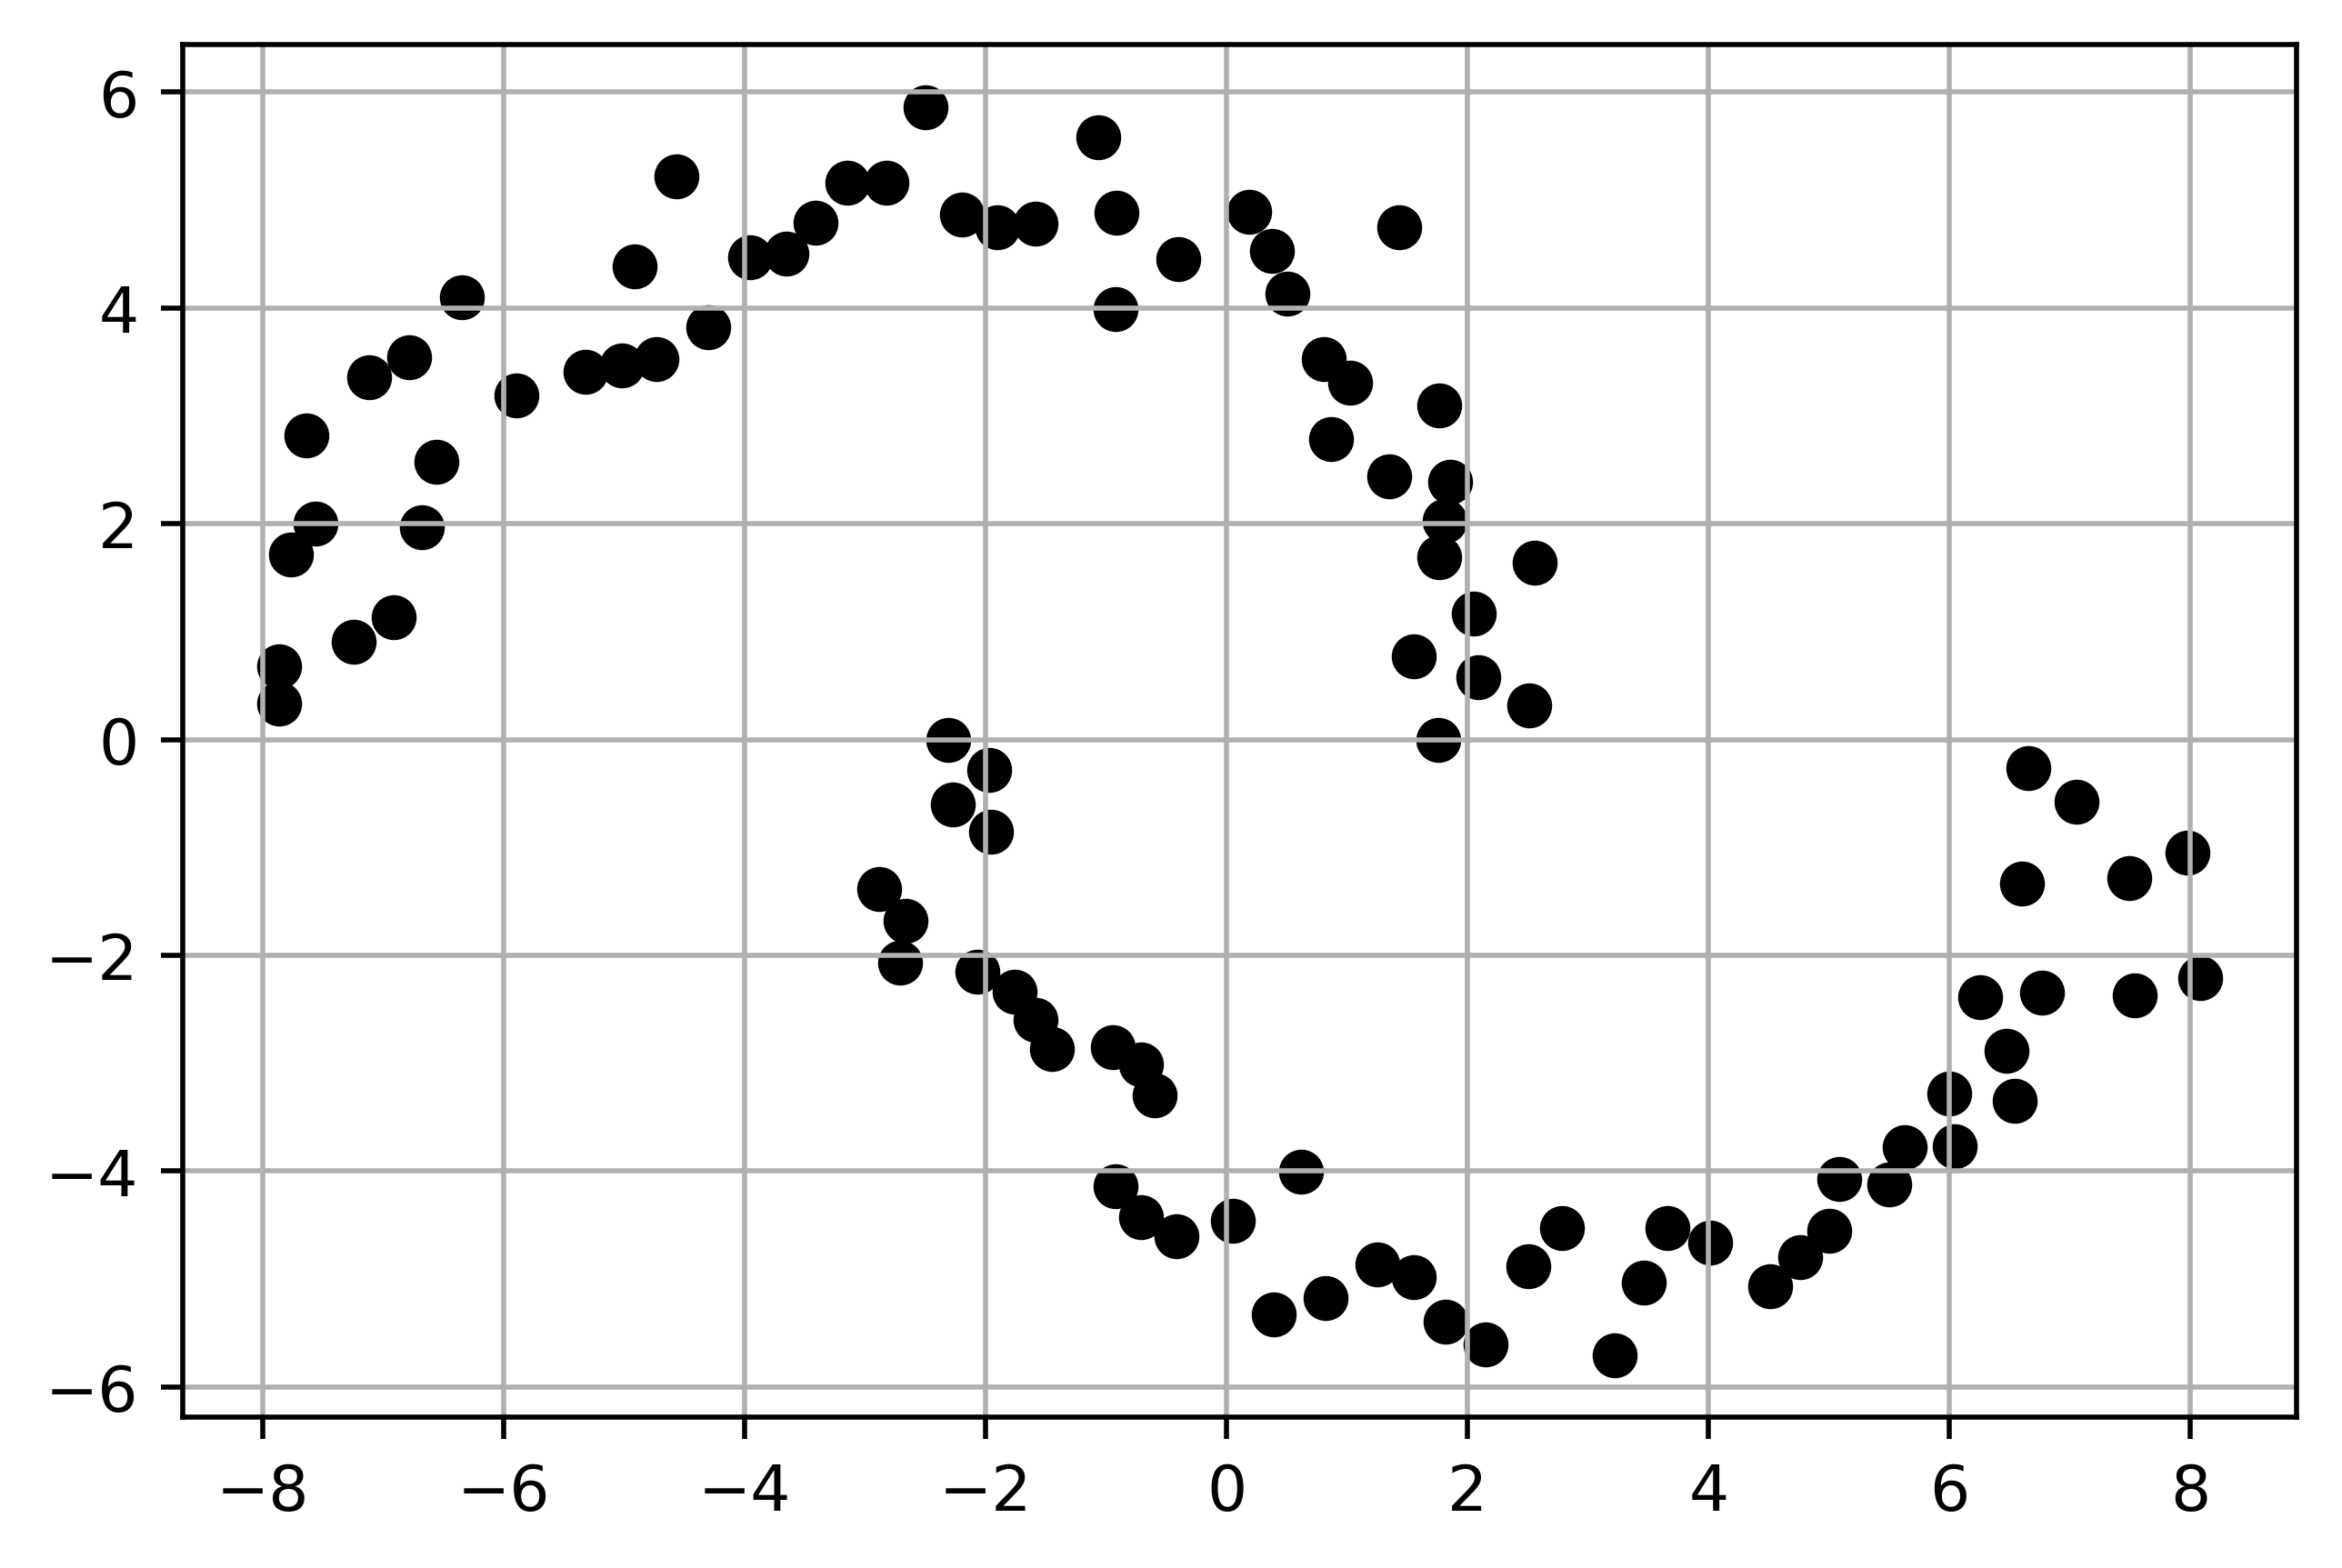
\includegraphics[width=0.65\textwidth]{images/clustering_images/offset_unclusterable.png}
            \caption*{This data can't be clustered either!}
        \end{figure}
        
        The edge of one cluster is too close to the other: we can't easily create a good pair of cluster means for each semi-circle.
        
\section{Terms}

    \begin{itemize}
        \item Clustering
        \item Unsupervised Learning
        \item Cluster
        \item Cluster mean
        \item $k$-means problem
        \item $k$-means loss
        \item Initialization
        \item Indicator Function
        \item Variance (Optional)
        \item $k$-means algorithm
        \item Hierarchical Clustering
        \item Consistency
        \item Ground Truth
        \item Visualization
        \item Interpretability
        \item Downstream Application
        \item Simpson's Paradox (Optional)
    \end{itemize}
    
    

%%%%%%%%%%%%%%%%%%%%%%%%%%%%%%%%%%%%%%%%%%%%%%%%%%%%%%%%%%%%%%%%%%%%%%%%%%%%%

 